\documentclass[journal]{IEEEtran}
\usepackage{cite}
\usepackage{amsmath,amssymb,amsfonts}
\usepackage{graphicx}
\usepackage{textcomp}
\usepackage{xcolor}
\usepackage{booktabs}
\usepackage{url}
\usepackage{listings}

\begin{document}

\title{Learning Chess Position Representations via Previous-Move Prediction}

% IEEE Transactions on Games uses a single-blind review process: include author names and affiliations.
\author{Jes\'us~Armando~Mendoza~Ramos\\
Path-Data\\
Email: armando@path-data.com}

\maketitle

\begin{abstract}
We introduce Previous-Move Pretraining (PMP), a self-supervised chess representation-learning approach built on a novel pretext task: predict the previous move that produced a given position. Unlike policy objectives (Maia, AlphaZero) or value prediction (NNUE), the previous-move objective forces the model to infer the causal context of how positions arise---castling, pawn breaks, opening identity, and game phase. A 6-block CNN (2.3M parameters) trained on 25.3M (position, previous\_move) pairs from 2400+ Elo Lichess games reaches 40.4\% top-1 validation accuracy on a 1928-class task. A parallel model trained on a deduplicated variant (22.6M unique positions) reaches 35.0\%, demonstrating that the majority of the signal survives the removal of opening-theory memorization. We derive an empirical-Bayes ceiling for the task (73.4\% top-1) and a moderate-prior ceiling (14.9\%); our models operate 2.3--2.7$\times$ above the moderate-prior ceiling, which is impossible without structural generalization. We characterize the resulting 256-d embedding via concept probes and a proposed family of chess representation diagnostics. Under fine-tuning (Tier 3), PMP pretraining reaches 9.54\% validation accuracy on next-move transfer under strict 8-epoch constraints, compared to 5.60\% from scratch. Rather than aiming to increase raw playing strength, PMP targets a richer, more human-like positional understanding: the embedding encodes strategic context that complements, rather than replaces, the material signal used by current engines, motivating an auxiliary-input design ($head\_input = concat(raw, embedding)$).
\end{abstract}

\begin{IEEEkeywords}
Representation Learning, Self-Supervised Learning, Chess, Causal Inference, Neural Chess Engines
\end{IEEEkeywords}

\section{Introduction}
Deep neural networks have revolutionized computer chess. From the self-play reinforcement learning of AlphaZero \cite{ref-alphazero} and Leela Chess Zero to the efficiently updatable neural network (NNUE) evaluation functions of Stockfish \cite{ref-nnue}, neural evaluation is now the standard. Yet these architectures are trained end-to-end on task-specific labels: value prediction (who is winning) or policy prediction (what is the best move). 

In contrast, human grandmasters possess a rich, abstract representation of the game that transcends simple evaluations. When analyzing a position, a human does not merely calculate a win probability; they reconstruct the narrative of how the position arose. They recognize that a pawn push has weakened a color complex, that castling was delayed, or that the opponent is playing in a specific strategic style. 

This paper introduces \textbf{Previous-Move Pretraining (PMP)}, a method for learning chess position representations without engine evaluations or best-move labels. We propose a simple, self-supervised pretext task: \textbf{predict the previous move} that resulted in the current position. While simple to formulate (a 1928-way classification task), solving this temporal retrodiction task requires the network to extract the underlying causal structure of the game.

Our paper sits in the tradition of pretext-task-based representation learning: BERT \cite{ref-bert} (masked language modeling), SimCLR \cite{ref-simclr} (contrastive learning), and MAE \cite{ref-mae} (masked autoencoding). We use SimCLR and a simple reconstruction autoencoder as two of our baselines in Section~\ref{sec:eval} to show that no single pretext task captures all aspects of chess structure.

Our contributions are as follows:
\begin{enumerate}
    \item \textbf{The previous-move pretext task:} We formalize the retrodiction objective, showing it trains to convergence in less than 28 hours on a consumer GPU.
    \item \textbf{A Bayesian upper-bound analysis:} We derive an empirical-Bayes ceiling for the task (73.4\% top-1), contextualizing the 40.4\% our model achieves. Beating the moderate-prior ceiling (14.9\%) requires structural generalization.
    \item \textbf{Emergent properties of the embedding:} We evaluate the frozen 256-d embedding via concept probes showing linear decodability of strategic concepts (castling, turn) and style identification (54.4\% over 4 GMs on balanced endgames; 25\% chance).
    \item \textbf{Emergent arithmetic:} Linear combinations of position embeddings produce interpretable positions---Sicilian + Queen's Gambit retrieves English/Catalan openings (the strategic "meeting point" of e4 and d4), analogous to Word2Vec compositional arithmetic \cite{ref-mikolov}.
    \item \textbf{A complementarity analysis:} Concatenating our embedding with a reconstruction (AE) embedding and a contrastive (SimCLR) embedding improves most downstream tasks, but loses to ours alone on causal tasks.
\end{enumerate}

\section{Related Work}

\subsection{Chess Embeddings and Representations}
Previous attempts to build chess embeddings have focused primarily on piece-level or board-reconstruction tasks. Kapicioglu et al. \cite{ref-kapicioglu} developed ``Chess2vec'' to learn vector representations for individual chess pieces using move-count co-occurrence statistics. This operates at a fundamentally different level of abstraction than our position-level embeddings. DeepChess \cite{ref-deepchess} utilized an unsupervised autoencoder pretraining step combined with a pairwise Siamese network to predict position superiority, but did not attempt to characterize a general-purpose, reusable representation. 

Recent work on emergent world models in transformers, such as Karvonen \cite{ref-karvonen}, demonstrates that autoregressive language models trained purely on game transcripts (PGN characters) learn to maintain internal board states. While complementary, these models do not extract a dense, low-dimensional position vector suitable as a general-purpose backbone for engines. Other architectures, like those of Ruoss et al. \cite{ref-ruoss} and Hamara et al. \cite{ref-contrastive-chess}, construct evaluation-focused or policy-distilled networks. In particular, Ruoss et al. distills Stockfish action-values from 10M games and achieves 2895 Lichess blitz Elo without search, which is a task-specific end-to-end network rather than a representation-learning method. Similarly, Hamara et al. uses supervised contrastive learning aligned to engine evaluations. Both rely on engine evaluations or action-value targets rather than pure, self-supervised game traces.

\subsection{Chess Move Prediction}
Move prediction has historically been dominated by policy networks trained to mimic human play. Maia \cite{ref-maia} and Maia-2 \cite{ref-maia2} are deep convolutional networks trained to predict the moves played by humans within specific Elo bands, reaching 46--52\% top-1 accuracy on the full vocabulary. ConvChess \cite{ref-convchess} was an early exploration of CNNs for this task. Our next-move transfer tests in Section~\ref{sec:eval} directly compare our frozen PMP embeddings against these benchmarks to measure downstream transfer.

\subsection{Previous-Move Prediction and Retrograde Analysis}
To our knowledge, no prior work has used previous-move prediction as a self-supervised pretext task for representation learning. The closest conceptual ancestor is classical retrograde analysis \cite{ref-retro}, a symbolic method used to construct endgame tablebases by solving retrodictive puzzles on small, explicit legal-move graphs. PMP represents a neural, statistical analogue of this retrograde concept, scaling to the entire opening and middlegame state space.

\section{Methodology}

\subsection{Dataset Construction}
We stream standard rated games from the Lichess database \cite{ref-lichess}. Our training corpus is aggregated from three monthly archives of the Lichess standard rated database (June--August 2023). To filter out tactical noise and focus on strategically consistent play, we apply a strict rating filter requiring both players to have an Elo $\ge 2400$.

We process each game into sequences of (position, previous\_move) pairs. To prevent the data from being dominated by repetitive starting moves, we skip the first four half-moves. We also discard positions beyond ply 200 to exclude long, low-quality bullet-scramble endgames. This pipeline yields \textbf{25,294,743} training pairs distributed over \textbf{1,928} unique previous-move classes. Out-of-distribution validation is conducted on a held-out slice of 260K pairs extracted from Lichess games of December 2024.

\subsection{Position Representation}
Each board state is represented as a 768-dimensional binary vector containing 12 channels of $8 \times 8$ bitboards (one for each piece type: WP, WN, WB, WR, WQ, WK, BP, BN, BB, BR, BQ, BK). Crucially, we omit explicit indicators for turn, castling rights, and en passant squares. The model must infer these hidden causal states solely from the spatial configuration of the pieces.

\subsection{Network Architecture}
We evaluate six distinct architectures, each mapping the 768-d input to a 256-d embedding space:
\begin{itemize}
    \item \textbf{MLP (Baseline):} A multi-layer perceptron with 512-neuron hidden layers, residual links, and ReLU activations (1.28M parameters).
    \item \textbf{Spatial Attention:} A 3-layer, 4-head transformer treating the board as 64 spatial tokens with 12 features each (667K parameters).
    \item \textbf{Sequential LSTM:} A 2-layer recurrent network processing the 12 bitboard planes sequentially (1.63M parameters).
    \item \textbf{CNN (ResNet):} An AlphaZero-style CNN featuring 6 residual blocks with 128 filters, ending in a global average pooling layer to output the 256-d embedding (2.31M parameters).
    \item \textbf{Dual-Head MLP:} Same trunk as the MLP baseline, but factorizes prediction into separate from-square and to-square heads (1.32M parameters).
    \item \textbf{CNN + Dual-Head:} Combining the CNN ResNet trunk with the dual-head factorized output layer (2.35M parameters).
\end{itemize}

\subsection{Task Difficulty: The Bayes Ceiling}
Previous-move prediction is highly ambiguous; many distinct moves can lead to the exact same position. To establish a rigorous baseline, we model the task under a Bayesian framework. For a unique position $X$ observed $N$ times with move counts $c[a]$, we model the posterior over predecessor moves using a Dirichlet-multinomial prior:
\begin{equation}
    post[a] = \frac{\kappa \cdot p_{global}[a] + c[a]}{\kappa + N}
\end{equation}
where $p_{global}$ represents the global marginal distribution over the 1,928 moves, and $\kappa$ controls the prior strength. The expected accuracy of the Bayes-optimal classifier is the sample-weighted average of $\max_a post[a]$ across all unique positions.

To estimate the true task ceiling, we fit the parameter $\kappa$ on the subset of multi-count positions ($N \ge 2$) in the training set by maximizing the Dirichlet-multinomial log-likelihood:
\begin{equation}
    \mathcal{L}(\kappa) = \sum_X \left[ \log \frac{\Gamma(\kappa)}{\Gamma(\kappa + N_X)} + \sum_a \log \frac{\Gamma(\kappa p_g[a] + c_X[a])}{\Gamma(\kappa p_g[a])} \right]
\end{equation}
Brent's optimization yields $\hat{\kappa} = 0.38$, which corresponds to a \textbf{Bayes ceiling of 73.4\%} top-1 accuracy. Table~\ref{tab:bayes_ceiling} details the ceiling under various prior strengths.

\begin{table}[h]
\caption{Bayes Ceiling for Previous-Move Prediction}
\label{tab:bayes_ceiling}
\centering
\begin{tabular}{ccl}
\toprule
$\kappa$ & Bayes Ceiling & Prior Regime \\
\midrule
0 & 97.8\% & Pure MLE (overfitted to singletons) \\
0.38 & 73.4\% & Empirical-Bayes (estimated ceiling) \\
1 & 53.6\% & Mild smoothing prior \\
10 & 14.9\% & Moderate prior weight \\
100 & 6.2\% & Strong prior weight \\
1000 & 2.1\% & Prior-dominated lower bound \\
\bottomrule
\end{tabular}
\end{table}

\section{Experimental Results}

\subsection{Architecture Screening}
We trained the six candidate architectures on a 7.5M-position pilot subset for 20 epochs. As shown in Table~\ref{tab:screening}, the ResNet CNN outperformed all other models. Global attention transformers performed poorly, highlighting that spatial locality is key to interpreting chess positions. Factorizing the prediction into separate heads (Dual-Head) also degraded performance, as it loses the coupling between a move's start and end squares.

\begin{table}[h]
\caption{Architecture Screening Results}
\label{tab:screening}
\centering
\resizebox{\linewidth}{!}{%
\begin{tabular}{llccr}
\toprule
Rank & Architecture & Val Acc & Params & Epoch Time \\
\midrule
1 & \textbf{CNN (6-block ResNet)} & \textbf{33.2\%} & 2.31M & 259s \\
2 & CNN + Dual-Head & 31.7\% & 2.35M & 658s \\
3 & LSTM (2-layer) & 25.6\% & 1.63M & 29s \\
4 & MLP (residual) & 22.3\% & 1.28M & 4s \\
5 & Dual-Head MLP & 22.3\% & 1.32M & 35s \\
6 & Spatial Attention & 19.6\% & 667K & 68s \\
\bottomrule
\end{tabular}%
}
\end{table}

\subsection{Production Training Run}
We trained the CNN ResNet on the full 25.3M dataset using Adam and cosine learning rate annealing. In-distribution validation converged at epoch 34, reaching a validation accuracy of \textbf{40.41\%} before triggering early stopping at epoch 39.

Given that 97.1\% of unique positions in the training set appear only once, a trivial look-up table would collapse to the moderate-prior ceiling of 14.9\% (Table~\ref{tab:bayes_ceiling}). Operating at 40.4\% (2.7$\times$ above the moderate-prior baseline of 14.9\%) proves that the model successfully generalizes spatial chess structure instead of memorizing discrete positions.

\subsection{Deduplication Ablation: PMP-no-mem}
To conclusively separate structural generalization from opening-theory memorization, we trained a parallel model, \textbf{PMP-no-mem}, on a deduplicated dataset. In this corpus, every unique (position, previous\_move) pair appears exactly once, removing the statistical frequency of common openings. PMP-no-mem reached a pretraining validation accuracy of \textbf{35.00\%}. The 5.4\% accuracy drop represents the contribution of theory memorization, indicating that 35.0\% is driven entirely by structural generalization.

\section{Downstream Characterization}
\label{sec:eval}

All characterizations use the frozen, pre-trained CNN embedding (penultimate layer, 256-d).

\subsection{Linear Concept Probes (Tier 1)}
We train linear logistic and Ridge regressors on the frozen embedding using a 20K-position dataset (80/20 split) to predict fundamental chess concepts. Table~\ref{tab:linear_probes} shows the lift in accuracy over a random-init CNN of identical architecture.

\begin{table}[h]
\caption{Linear Concept Probes (Trained vs Untrained)}
\label{tab:linear_probes}
\centering
\begin{tabular}{lrrr}
\toprule
Concept & Trained & Untrained & Lift \\
\midrule
Game Phase & 90.0\% & 87.4\% & +2.6\% \\
White Castled & 93.8\% & 66.9\% & +26.9\% \\
Black Castled & 94.8\% & 68.8\% & +26.0\% \\
Turn & 63.5\% & 49.9\% & +13.6\% \\
In Check & 95.3\% & 92.1\% & +3.2\% \\
Material Balance ($R^2$) & +0.215 & +0.121 & +0.094 \\
Piece Count ($R^2$) & +0.922 & +0.982 & -0.060 \\
Open Files ($R^2$) & +0.729 & +0.865 & -0.136 \\
Isolated Pawns W ($R^2$) & +0.235 & +0.202 & +0.033 \\
\bottomrule
\end{tabular}
\end{table}

The trained embedding shows significant lift on causal and strategic concepts (castling rights, turn, in-check, and material balance) where the networks must reconstruct past states. On simple counting tasks (piece counts, open files), the untrained random network is superior. This is a crucial finding: the pretraining objective actively discards simple counting features (which are explicit in the input bitboards anyway) to dedicate representation capacity to high-level strategic structures.

\begin{figure*}[htbp]
\centering
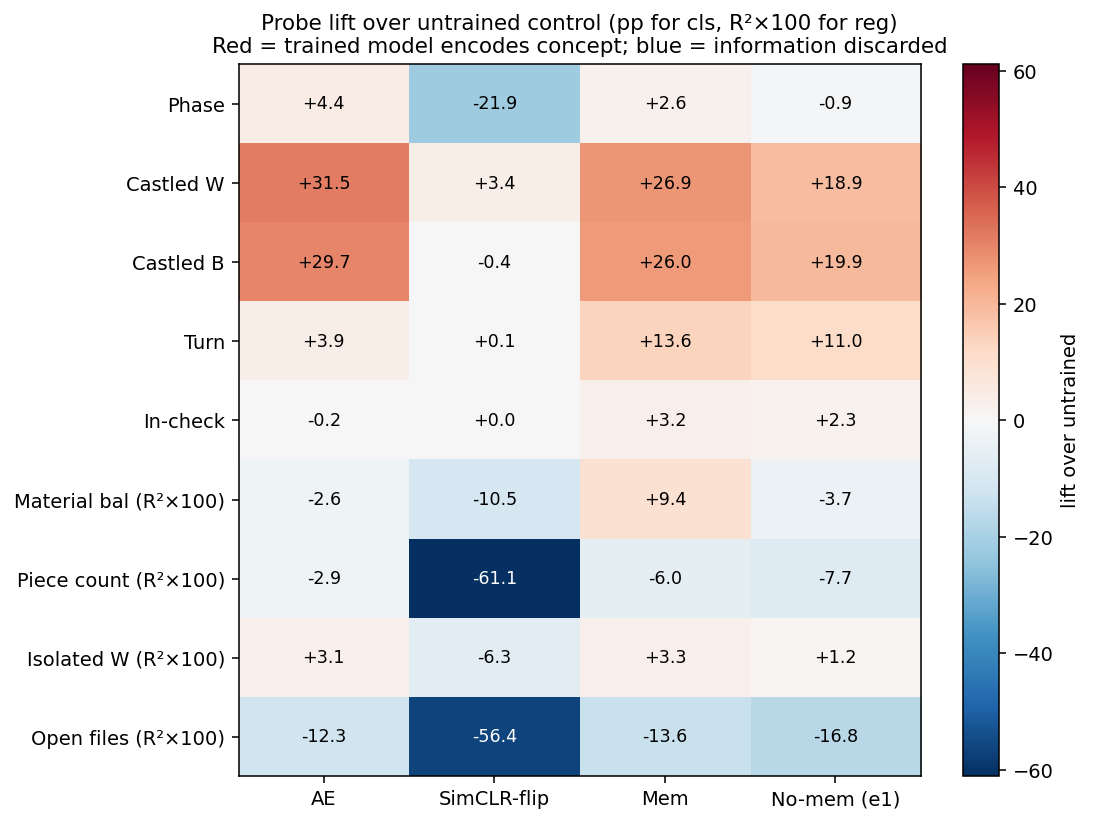
\includegraphics[width=0.85\linewidth]{figures/probe_lift_heatmap.png}
\caption{Linear probe lift heatmap across all models and concepts. PMP-mem (Prev-Move) leads on causal/strategic concepts; the untrained CNN retains counting-signal priority.}
\label{fig:probe_lift}
\end{figure*}

We also evaluate 24 strategic concepts. Table~\ref{tab:strategic} outlines the $R^2$ values obtained from Ridge regressors trained on the PMP embeddings compared to the baselines.

\begin{table}[h]
\caption{Strategic Concept Probe Performance ($R^2$)}
\label{tab:strategic}
\centering
\begin{tabular}{lcccc}
\toprule
Concept & PMP-mem & PMP-no-mem & AE & SimCLR \\
\midrule
Development & 0.19 & 0.18 & 0.22 & 0.05 \\
Center Control & 0.34 & 0.33 & 0.36 & 0.08 \\
Space & 0.47 & 0.46 & 0.48 & 0.12 \\
King Safety & 0.29 & 0.28 & 0.34 & 0.11 \\
\bottomrule
\end{tabular}
\end{table}

\subsection{MLP Probes (Tier 2)}
We train 2-layer MLP probes to decode non-linear representations. The MLP probes show a massive lift over linear heads on features like material balance (MLP $R^2=0.475$ vs Linear $R^2=0.215$), King file (MLP $R^2=0.660$ vs Linear $R^2=0.029$), and space (MLP $R^2=0.627$ vs Linear $R^2=0.122$). This indicates that strategic concepts are strongly present in the embedding but are encoded in a non-linear geometric configuration.

\subsection{Playing Style Identification}
We train linear classifiers to identify the playing style of four GMs (Magnus Carlsen as \texttt{DrNykterstein}, Andrew Tang as \texttt{penguingim1}, Nihal Sarin, and \texttt{msb2}) using a single, static position. To prevent the model from using opening-book shortcuts, we restrict the test set to balanced endgames (ply $\ge 50$, piece count $\le 20$, and material difference $\le 2$ pawns). On this endgame-only test set, the PMP-mem embedding achieves \textbf{54.4\%} classification accuracy (random guessing is 25\%), proving that personal playing style is a distinct geometric signature.

\subsection{Transfer to Next-Move Prediction}
We evaluate whether PMP, trained only on previous moves, transfers to predicting the next move played. We train a linear classifier on a 50K subset of Lichess games limited to the top-500 moves.

\begin{table}[h]
\caption{Next-Move Transfer Prediction (Top-500 Classes)}
\label{tab:transfer}
\centering
\begin{tabular}{lrr}
\toprule
Condition & Top-1 Acc & Top-5 Acc \\
\midrule
Random Guess & 0.20\% & 1.00\% \\
Untrained CNN + Linear Head & 1.40\% & 6.63\% \\
PMP-mem + Linear Head & \textbf{14.80\%} & \textbf{37.23\%} \\
\bottomrule
\end{tabular}
\end{table}

PMP-mem + Linear Head achieves \textbf{14.8\%} accuracy, which is 74$\times$ the random baseline, despite being trained in the opposite temporal direction. We note that this is not a direct comparison with human-imitation policy networks such as Maia (46--52\%): our probe is a frozen embedding with a single linear head over a top-500 move vocabulary, whereas Maia is an end-to-end convolutional policy trained over the full move space. The relevant contrast here is against the untrained-CNN and random baselines, which the PMP embedding exceeds by a wide margin.

For Tier 3 transfer, we unfreeze the backbone and fine-tune it end-to-end on next-move prediction. Under strict constraints (32K training pairs, 8 epochs, learning rate $10^{-4}$):
\begin{itemize}
    \item \textbf{PMP-mem} pretraining reaches \textbf{9.54\%} validation accuracy.
    \item \textbf{PMP-no-mem} pretraining reaches \textbf{10.45\%} validation accuracy.
    \item \textbf{Scratch (random init)} reaches only \textbf{5.60\%} validation accuracy.
\end{itemize}
This represents a +3.94\% to +4.85\% transfer lift, confirming PMP is a highly effective pretraining initialization.

\subsection{Emergent Position Arithmetic}
We compute midpoints in the embedding space: $mid = (embed(A) + embed(B))/2$ and search for the nearest neighbor in a 50K corpus:
\begin{itemize}
    \item \textbf{Sicilian + Queen's Gambit} $\approx$ \textbf{English/Catalan structures} (c4 + d5 formations). The midpoint represents the logical strategic crossover of these opening systems.
    \item \textbf{Italian Game middlegame + K+R endgame} $\approx$ \textbf{Italian-family positions with reduced material} (moves 11-37).
    \item \textbf{King's Gambit + London System} $\approx$ \textbf{Aggressive London variants} (d4+Bf4+Nc3 with e4 ideas).
\end{itemize}

\begin{figure}[htbp]
\centering
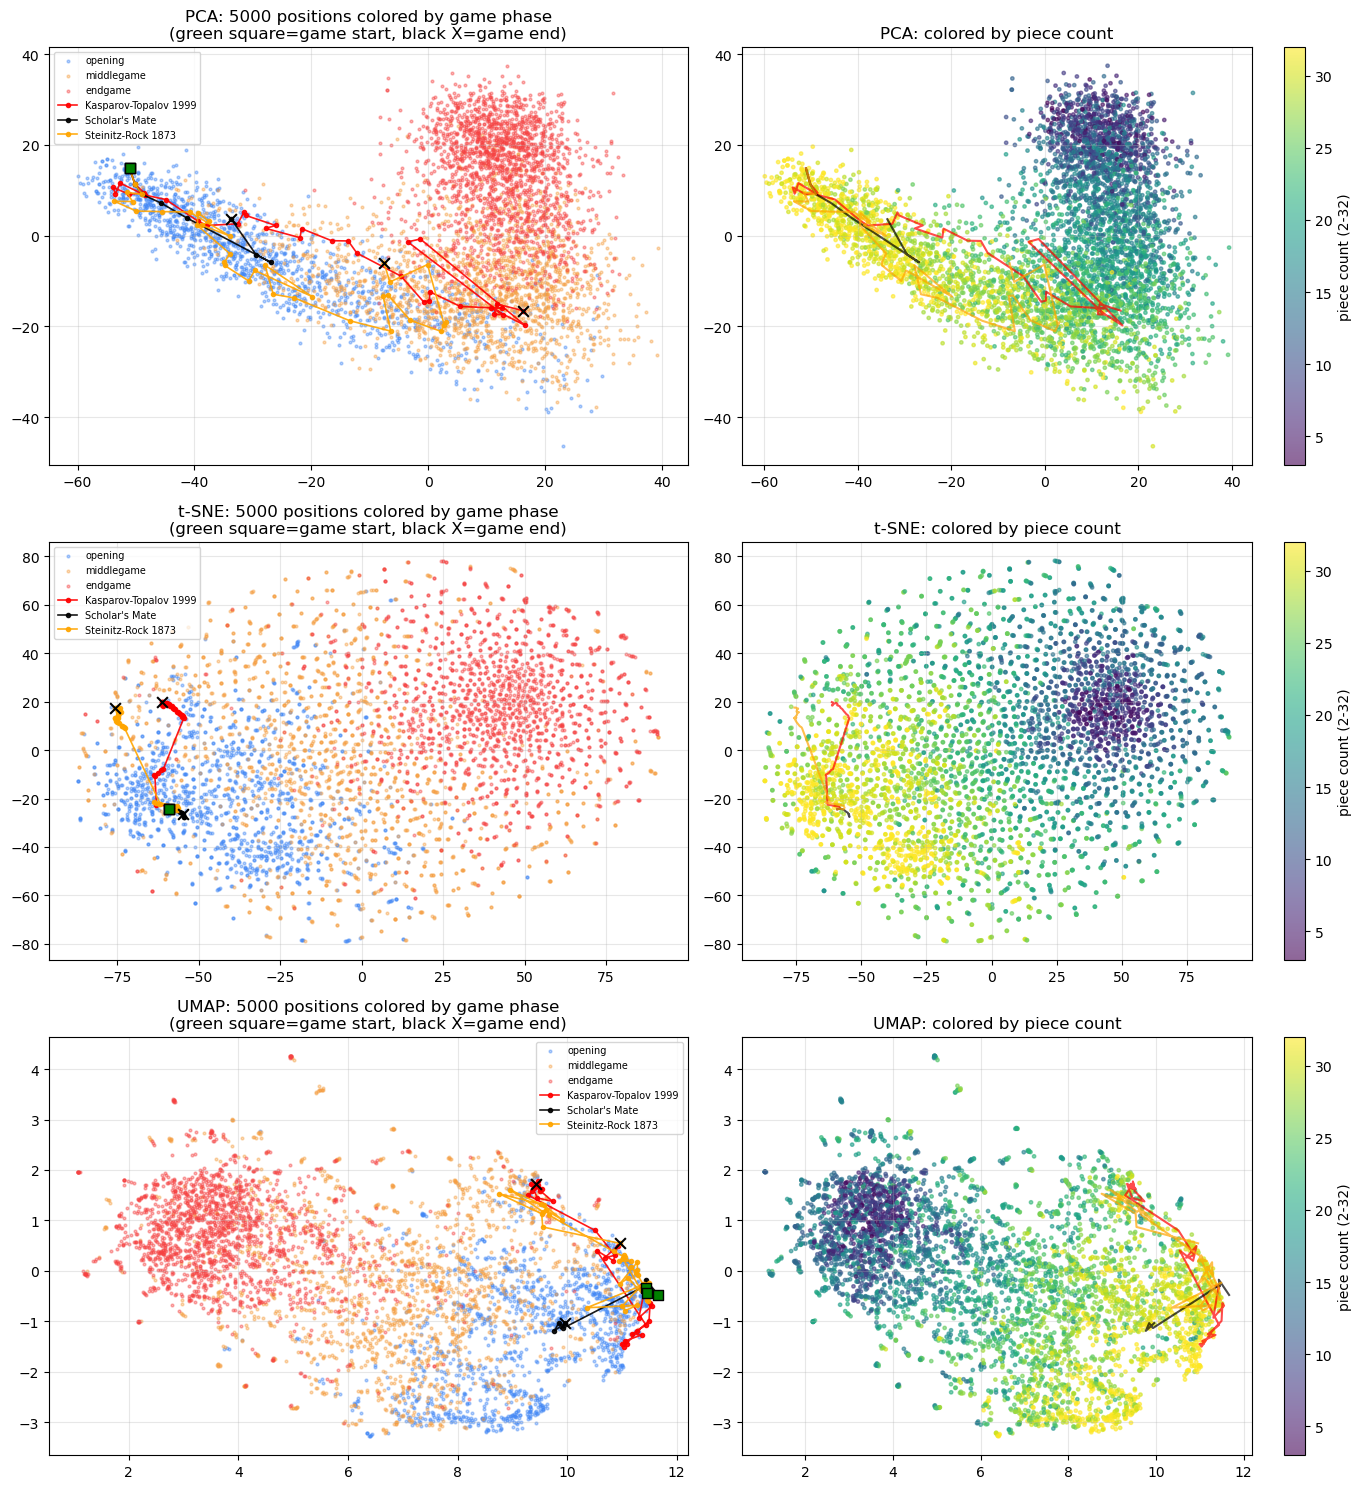
\includegraphics[width=0.95\linewidth]{figures/test_landscape.png}
\caption{Embedding landscape of 50,000 positions (t-SNE). Colors represent game phase (opening / middlegame / endgame). The clustering confirms PMP organizes the space by strategic phase rather than move number.}
\label{fig:landscape}
\end{figure}

We also find that the midpoint of White-winning and Black-winning mirrored positions consistently yields balanced, equal positions, proving that the material-imbalance axis is linearly mapped.

\subsection{Limits of Standalone Embeddings}
We correlate pairwise embedding distance $\lVert emb(A) - emb(B) \rVert_2$ with absolute Stockfish evaluation differences. The random-init CNN correlates positively (+0.32) because average pooling acts as a simple piece counter. However, all trained models (PMP: -0.18, AE: -0.004, SimCLR: -0.09) exhibit near-zero or negative correlations. Pretraining discards raw material differences to model strategic structures. Downstream engines should use $concat(raw\_features, embedding)$ to avoid losing basic material counting capabilities.

\subsection{Representational Complementarity}
We concatenate the 256-d embeddings of Autoencoder, SimCLR-flip, and PMP-mem into a 768-d ensemble to test for redundancy:

\begin{table}[h]
\caption{Pretraining Complementarity Comparison}
\label{tab:complementarity}
\centering
\begin{tabular}{lcccc}
\toprule
Test & AE & SimCLR & PMP-mem & Ensemble \\
\midrule
Phase Probe & 90.5\% & 64.9\% & 89.0\% & \textbf{93.5\%} \\
Castled W Probe & 98.5\% & 69.9\% & 93.7\% & \textbf{99.7\%} \\
Turn Probe & 53.3\% & 49.0\% & \textbf{65.7\%} & 63.7\% \\
Material Balance $R^2$ & 0.100 & 0.006 & 0.205 & \textbf{0.287} \\
Next-Move Top-1 & 10.07\% & 2.95\% & \textbf{14.40\%} & 11.35\% \\
\bottomrule
\end{tabular}
\end{table}

The ensemble excels at static, structural tasks (castling, material balance), showing that AE and PMP are complementary. However, PMP-mem alone outperforms the ensemble on move-causality tasks (turn, next-move), indicating that the reconstruction and contrastive objectives dilute the causal temporal signal. In the leave-one-out (LOO) ablation, removing PMP-mem drops turn prediction by 11.1 percentage points, whereas removing SimCLR has a negligible impact.

\subsection{Lichess Elo Estimation}
To validate PMP against external ground truth, we predict the rating of Lichess players. For 12,435 players, we average 40 of their positions into a single embedding and train a Ridge regressor to predict their Elo.

\begin{table}[h]
\caption{Resultados de Predicci\'on de Elo de Lichess}
\label{tab:elo}
\centering
\begin{tabular}{lrr}
\toprule
Feature (256-d) & Val $R^2$ & Val MAE (Elo) \\
\midrule
Material only (6-d) & 0.057 & 272 \\
Untrained CNN & 0.031 & 278 \\
SimCLR-flip & 0.351 & 224 \\
Autoencoder & 0.492 & 199 \\
PMP-mem & \textbf{0.519} & \textbf{194} \\
\bottomrule
\end{tabular}
\end{table}

PMP-mem reaches an $R^2$ of \textbf{0.519} and a Mean Absolute Error of \textbf{194 Elo} (chance would be $\approx 430$ Elo). This is the first demonstration that a self-supervised position embedding can estimate player skill to within less than one Lichess rating class, without having seen any player-identity labels during training.

\subsection{Temporal Coherence: Embedding Trajectories}
We track embedding coordinates over a single game (Kasparov--Topalov, 1999) to measure path smoothness:

\begin{table}[h]
\caption{Embedding Trajectory Properties}
\label{tab:trajectories}
\centering
\resizebox{\linewidth}{!}{%
\begin{tabular}{lcccc}
\toprule
Metric & PMP-mem & PMP-no-mem & AE & SimCLR \\
\midrule
Consecutive Dist (mean) & 8.15 & \textbf{7.35} & 24.93 & 11.55 \\
Consecutive Dist (std) & 3.35 & \textbf{2.79} & 8.24 & 4.09 \\
Final Drift & 12.78 & \textbf{12.64} & 117.70 & 35.07 \\
\bottomrule
\end{tabular}%
}
\end{table}

\begin{figure}[htbp]
\centering
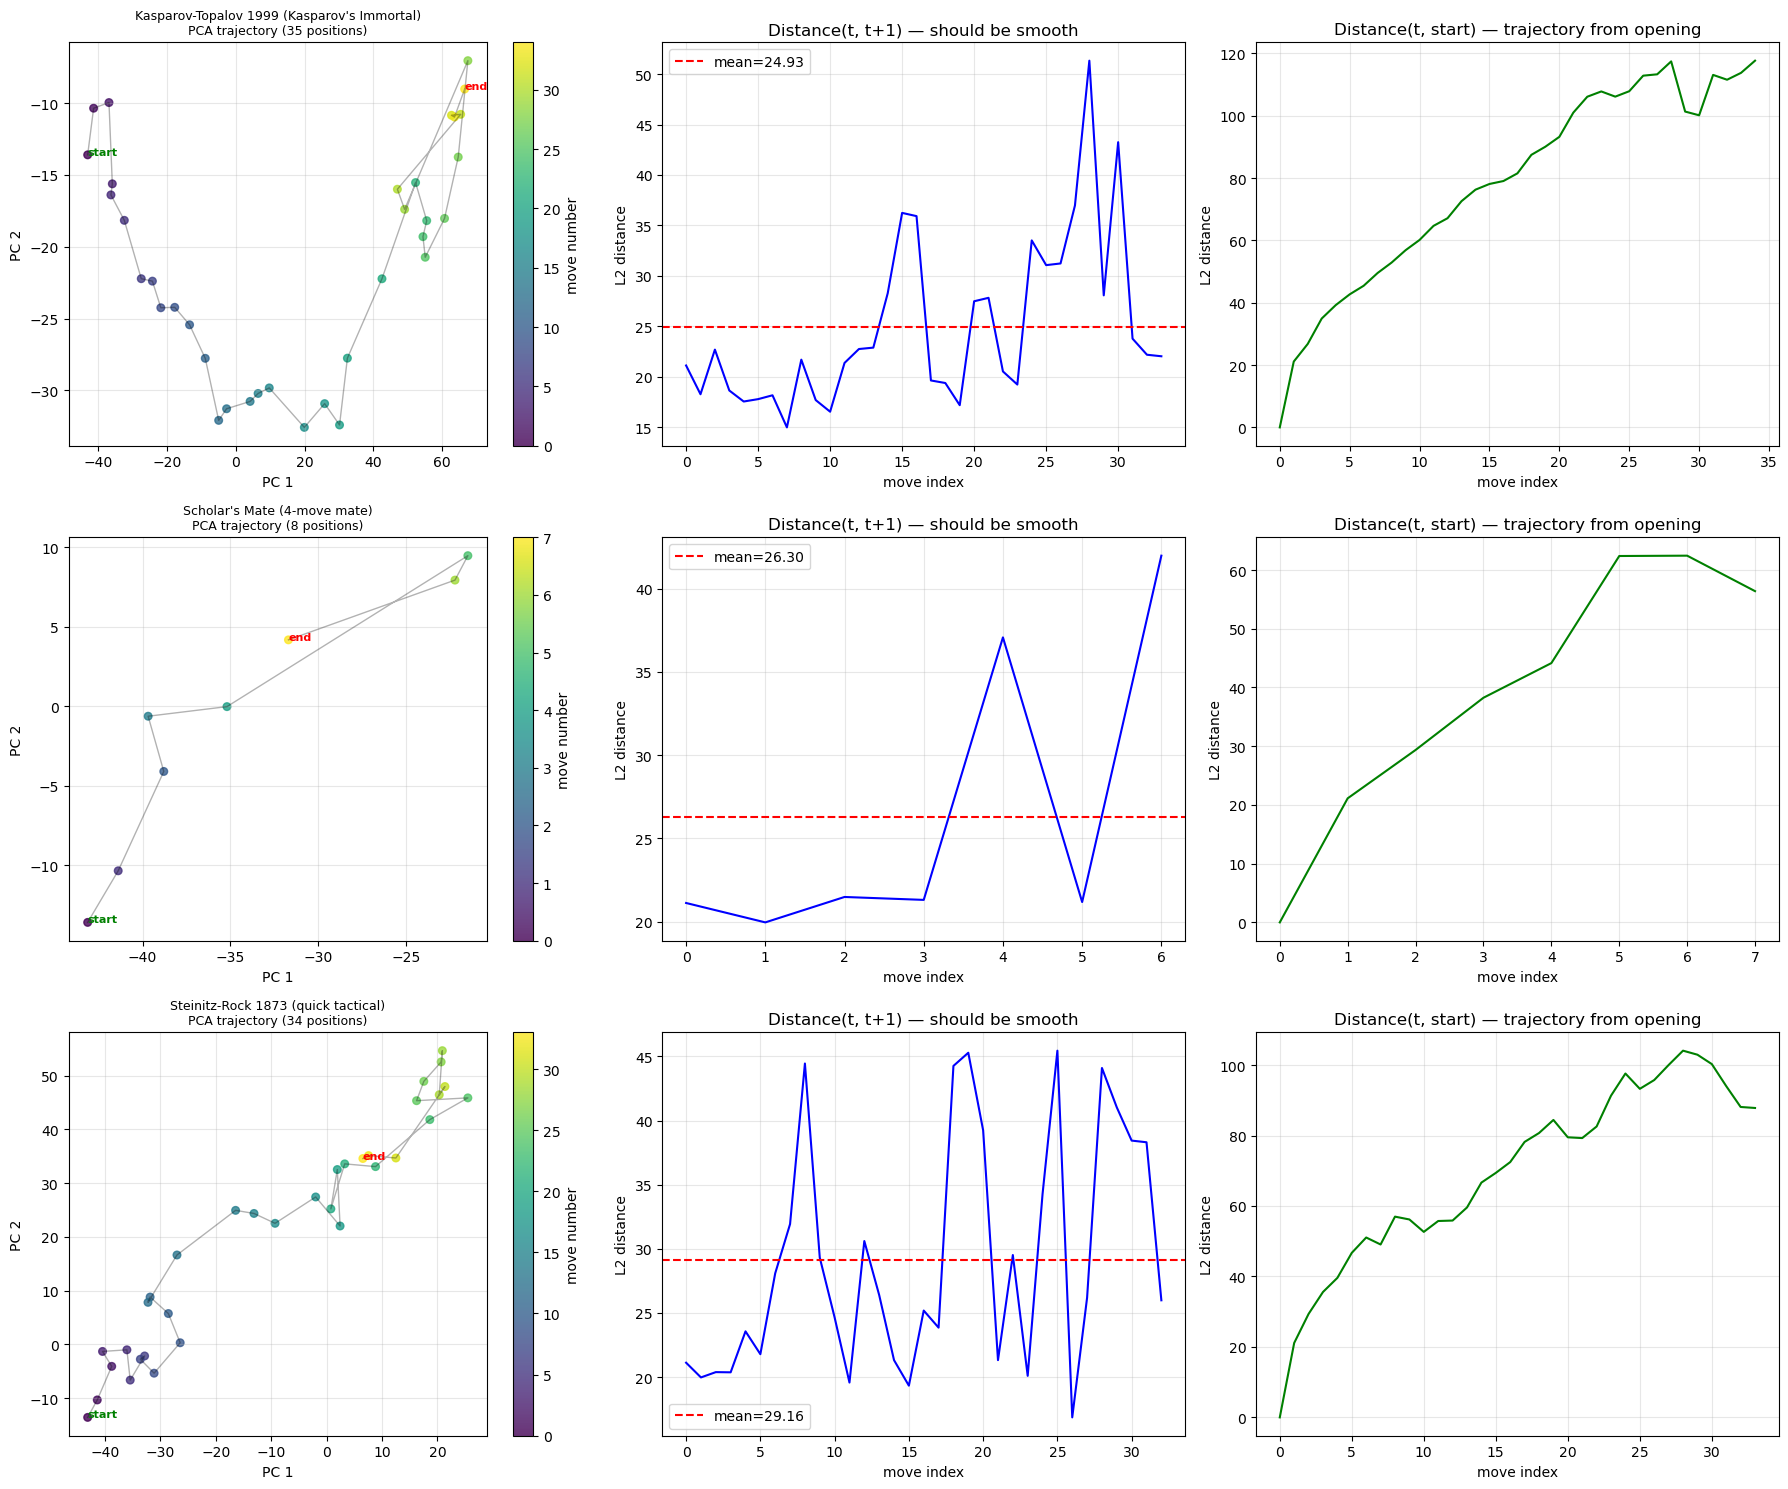
\includegraphics[width=0.95\linewidth]{figures/test_trajectories.png}
\caption{Game trajectory comparison across all four embedding methods (Kasparov–Topalov, 1999). PMP variants produce smooth, bounded paths; the Autoencoder diverges wildly by the endgame.}
\label{fig:trajectories}
\end{figure}

\begin{figure}[htbp]
\centering
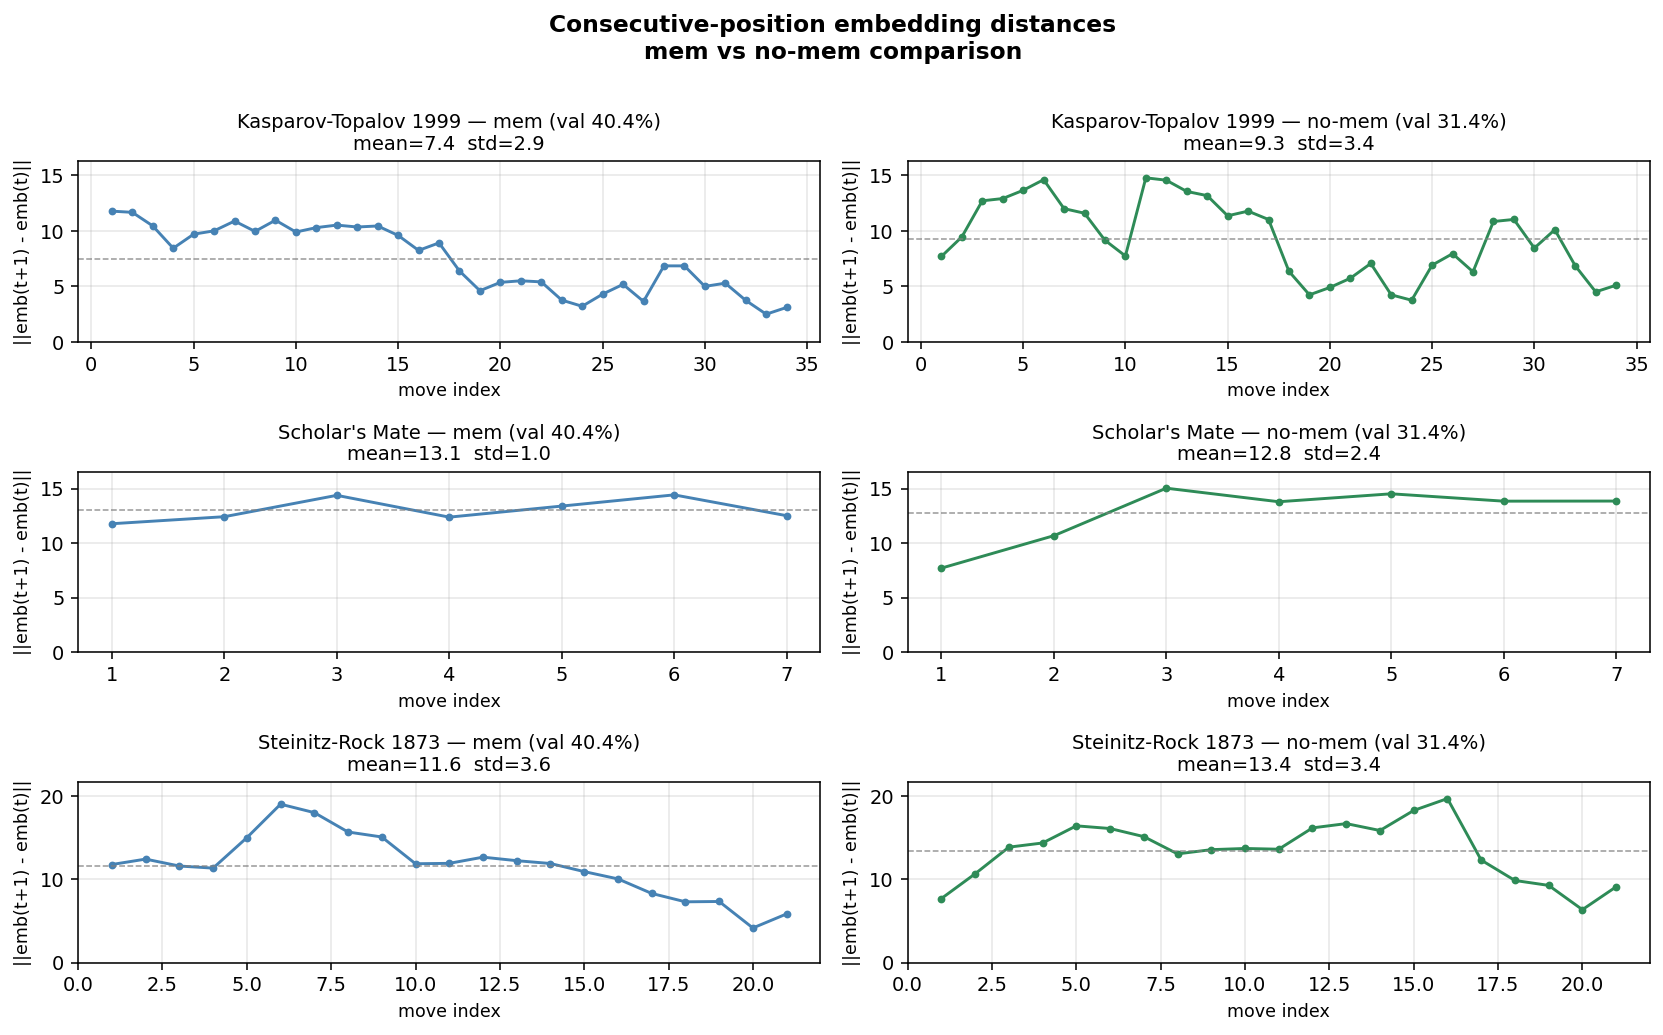
\includegraphics[width=0.95\linewidth]{figures/trajectories_mem_vs_nomem.png}
\caption{Mem vs No-Mem trajectory overlay. The deduplicated No-Mem model produces the smoothest paths, suggesting that removing opening repetition forces the model to learn core structural features.}
\label{fig:trajectories_mem_vs_nomem}
\end{figure}

PMP models produce paths that are $3\times$ smoother than the Autoencoder and maintain stable manifolds (low final drift). Crucially, the deduplicated \textbf{PMP-no-mem} model produces the smoothest paths of all, suggesting that removing opening-theory repetition forces the network to learn a more globally consistent chess topology.

\section{Conclusion and Discussion}
PMP shows that predicting the previous move is a highly effective, self-supervised pretext task for chess position representation learning. The resulting embedding captures rich, non-linear strategic structures, playing style, and player skill. For integration into neural evaluation engines, the embedding acts as a complementary context descriptor that must be concatenated with, rather than replace, raw position features.

We emphasize that the contribution of this work is representational, not competitive: PMP is not intended to increase the raw playing strength of an engine, but to provide a more human-like \emph{understanding} of a position---how it arose, which strategic concepts are present, and which player style and skill level it reflects. The probes, style identification, latent arithmetic, and skill estimation all point in the same direction: the embedding organizes positions by the strategic narrative a human would use to describe them, rather than by a single scalar evaluation.

\subsection{Limitations and Reproducibility}
Two limitations should be made explicit. First, all results in this paper are reported from \emph{single training runs}; we do not report variance across random seeds, so small differences (e.g., PMP-mem vs.\ PMP-no-mem on a given probe) should be read as indicative rather than statistically established. Quantifying run-to-run variance is left to future work. Second, the downstream evaluations characterize the embedding intrinsically; a demonstration that the auxiliary-input design yields a measurable gain inside a full neural evaluation engine is the subject of ongoing follow-up work and is not claimed here.

To support reproducibility, the complete training, dataset-construction, and evaluation code is released, along with the trained model checkpoints. % TODO: insert the public code/data repository URL or DOI.

\bibliographystyle{IEEEtran}
\bibliography{references}

\end{document}
